
%: ----------------------- introduction file header -----------------------
% the code below specifies where the figures are stored
\graphicspath{{4/figures/}}

\chapter{Timbre Similarity}
\label{chp:timbre}

% Context
Timbre has proven to be a difficult attribute to define in acoustic perception, and there is little concensus as result in its underpinnings or the efforts to model it computationally.
% Purpose
Psychoacoustics has long sought to better understand the space of timbre using subjective pairwise ratings between acoustic stimuli, but this information is costly to obtain and the generalizability of conclusions ultimately dependent on the palette of sounds considered.
% Goal
This chapter explores an objective, data-driven approach to the development of relative timbre spaces as a scalable alternative to this line of research.
% Approach / how
Here, instrument taxonomies are used to as a proxy for timbre similarity, and a deep convolutional network is used to project time-frequency representations of audio into a low-dimensional, semantically organized space.
The quality of the resulting embeddings is demonstrated through a series of experiments, indicating that this approach shows significant promise for organizing large collections of audio samples by timbre.


\section{Context}
\label{sec:context}

% Definition
Despite its common usage in the various forms of music for centuries, a satisfactory definition of \emph{timbre} remains elusive to this day; in fact, the one adopted by the American National Standards Institute embodies this challenge, arriving at a concept through the exclusion of others \cite{ANSI197x}:

\begin{quote}
Timbre is that attribute of auditory sensation in terms of which a subject can judge that two sounds similarly presented and having the same loudness and pitch are dissimilar.
\end{quote}

%  More focus on what it isn't than what it is
As evidenced by this definition, the very notion of ``timbre'' is still an open research topic in psychoacoustics.
This reality is captured quite succinctly by Phillipe Manoury, who offered the following insight \cite{Manoury19XX}:

\begin{quote}
One of the most striking paradoxes concerning timbre is that when we knew less about it, it didn’t pose much of a problem.
\end{quote}

% Why is this problematic
There are many advantages to developing a deeper understanding of timbre, from both an artistic and scientific perspective.
Of particular interest to this work, however, the absence of a constructive definition ---timbre is a result of X, Y, and Z--- makes it difficult to directy build computational systems to characterize and compare timbres.
Thus, before proceeding, it is valuable to review what is known of timbre, and prior efforts to transfer this knowledge into engineering systems.
% There is much to be understood about "timbre"; point is, question everything we think we know.


\subsection{Psychoacoustics}
% Historical context
% Psychoacoustics, Early work and the struggle to define
% Helmholtz, pitch, and other psychoacoustics.
%Given this inherent ambiguity in concept definition, it is worthwhile to contextualize how this situation came to be.
The perception of timbre falls under the umbrella of \emph{psychoacoustics}, a topic of study that sits at the boundary between acoustics and psychology.
Some of the earliest research in psychoacoustics was pioneered by von Helmholtz in his inquiries into the sensations of pitch and loudness \cite{Cook1995?}.
Inquiries specific to timbre would not come until much later, due to two difficulties in experimental design.
One, whereas pitch and loudness can be ranked on a one dimensional scale, it is unclear from personal introspection what the salient dimensions of timbre might be.
Instead, it is often necessary to use methaphors as a means of comparing and relating the perception of timbre, such as describing a sound as ``bright'' or ``muddy''.
Additionally, researchers were limited by the kinds of stimuli they could create and use in perceptual experimentation, and thus were constrained in the space of possible parameters to explore.

% Psychology and psychoacoustics in the 1960-90s
With the advent of computers and continued scientific advances through the 20th century, these issues could be addressed directly, and several researchers set out to identify the existence of fundamental dimensions.
This work, perfomed by Plomp \cite{Plomp1976} Grey and Wessel \cite{Grey1979}, among others, adopted a similar experimental design.
Human subjects are presented pairs of sound stimuli and asked to rate the similarity between the two.
Having collected an exhaustive set of pairwise ratings from a number of participants, multi-dimensional scaling is then used to project the stimuli into a low-dimesional space such that the reported relationships between these datapoints are minimally distorted \cite{Grey1979}; an example space is shown in Figure \ref{fig:grey_mds}.
Using this similarity model, the researcher then considers a wide array of time-frequency signal statistics, or \emph{features}, in order to identify those that best correlate with the different dimensions.
% Outcomes
This approach has produced a useful, albeit large, set of features on which computational models have been constructed.
Among the earliest were those of log-attack time, spectral centroid, and spectral spread, and were later corroborated by other researchers, as in the work of Krumhansl \cite{Krumhansl}.

\begin{figure}[t]
\centering
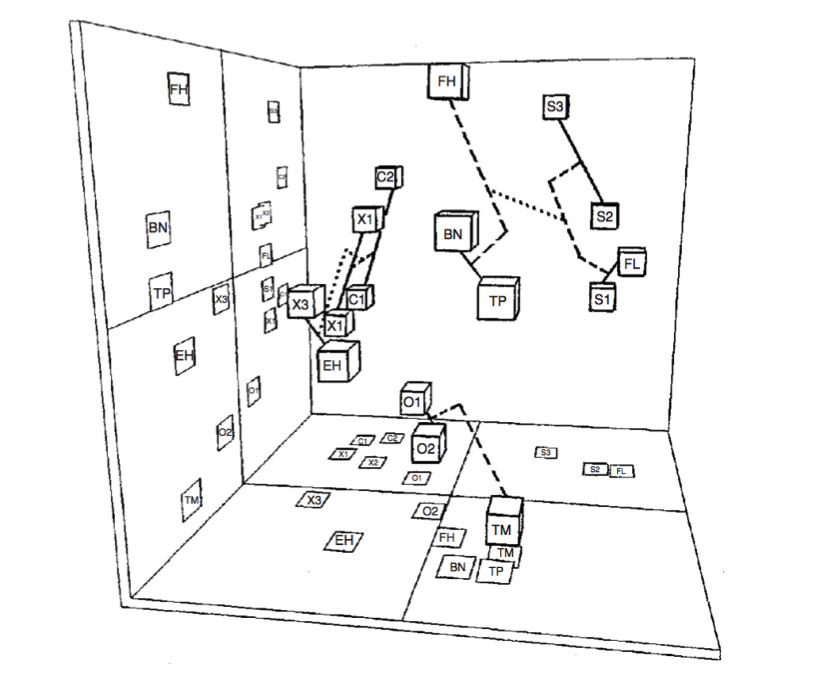
\includegraphics[width=\textwidth]{grey-mds.png}
\caption{The resulting MDS model developed in the work of Grey and Wessel.}
\label{fig:grey_mds}
\end{figure}

% This line of inquiry showed promise, and went on to inform much of how MIR approaches timbre and how such systems should be built.

% Deficiencies
%  - subjective ratings are limited by the space of stimuli used
%  - researcher must dig in to find different features for every model
%  - costly to obtain ratings
More recently, however, some have begun to recognize a few shortcomings of this approach to timbre research \cite{Glennon2014}.
First, a timbre space derived from the multidimensional scaling of pairwise ratings is limited to the sonic palette used to produce it, and the inclusion of additional stimuli is likely to rearrange how the space is organized.
For instance, the MDS model for a collection of orchestral instruments will be quite different with and without considering electronic synthesizers.
This also has significant implications on the granularity of sounds considered.
In \cite{Krumhansl1980?}, the attack and sustained regions of a sound were considered separately, resulting in slightly different MDS models.
% Additionally, concatenating the attack of one instrument with the sustained portion of another would cause a subject to perceive only the attack instrument.
This is not to say that a space derived from relative comparisons is necessarily deficient, however, simply that it must be adapted in the presence of new or different information.
Second, the process of finding well-correlated features to explain the resulting MDS model is difficult and time consuming.
A researcher must repeat the involved process of feature exploration for every model obtained through a different combination of stimuli.
Furthermore, as noted by Caclin et al., ``Given the multiplicity of acoustical parameters that could be proposed to explain perceptual dimensions, one can never be sure that the selected parameters do not merely covary with the true underlying parameters.'' \cite{Caclin2005}.
In other words, correlation does not imply causation, and features identified by inspection entail some degree of uncertainty.
Finally, the process of collecting subjective pairwise ratings is especially costly, because the number of possible comparisons increases quadratically with number of unique stimuli considered.
This places a practical constraint on the generality of a timbre space, as it quickly becomes impossible for subjects to exhaustively rate all combinations.
In the absence of complete information, statistical methods, such as imputation, are necessary to interpolate a sparse set of responses.


%Synthesizing this brief survey of timbre perception research into some kind of workable defintion, timbre is a time-varying quality of sound, akin to texture in the visual domain.
% Referred to by Landy as a \emph{second-order percept}, texture is the emergent property

% What are the take-aways here?
% - Previous claims of salient dimensions should be taken with a grain of salt.
% - This is why we are where we are.


\subsection{Computational Modeling of Timbre}
% Computational approaches and models
% Short-time statistics
Most previous approaches to computationally modeling timbre instantaneously can be grouped into one of two categories: signal statistics and basis projections.
The first follows from the perceptual research described above, whereby specific features are designed to encode some high level semantic concept, e.g. log-attack time or spectral brightness.
Initially these corresponded to the features named by in the work of Grey or Krumhansl, but have expanded over time to include a wide array of creative and clever measures.
The interested reader is directed to \cite{Essid2006} for a comprehensive space of possible features.

% Cascaded Transforms
From an often complementary perspective, other music researchers have utilised transform-based approaches to project signals into representations with various desirable properties.
One of the earliest and most common approaches is the use of Mel-frequency Cepstral Coefficients (MFCCs) for timbre-oriented tasks.
Originally designed for speech coding by Mermelstein et al in the 1960s \cite{Mermelstein}, the first significant contribution in MIR to call attention to MFCCs as useful music features was that of Logan in 2000 \cite{Logan}.
MFCCs have, at least in practice, become nearly synonymous with timbre-centric MIR, now being used in a wide array of systems for instrument classification \cite{anyone}, tagging \cite{anyone_else}, genre prediction \cite{jesus}, mood estimation \cite{schmidt} or structural analysis \cite{levy}, to name only a few representative works in each.
As described in detail in Chapter \ref{chapter:context}, the general process of computing MFCCs proceeds as follows: an input audio signal is divided into overlapping, short-time \emph{frames}, on the order of tens to hundreds of milliseconds; a filterbank, perceptually scaled in frequency, is then applied to each short-time frame and log-compressed; finally, a discrete cosine transform (DCT) is applied to these frequency coefficients, characterizing the shape of the spectrum (or the spectrum of the spectrum, referred to as the \emph{ceps}trum).
Only the first dozen or so coefficients are used, based on the principle that they compactly describe the spectral contour, though this is more convention than rule.
Some have even gone so far as to literally \emph{equate} MFCCs and timbre, concluding that specific coefficients are responsible for various perceptual dimensions \cite{Teresawa2007}.

% Machine learning approaches
Similar in principle, though less widely adopted, is to instead \emph{learn} the set of bases against which a time-frequency representation is projected.
One such instance is observed in  \cite{Jehan2005}, which preserves the first 12 coefficients of a trained PCA decomposition.
In this scenario, the projection into the PCA subspace serves to decorrelate the principal axes of the data in the input space, much like the Discrete Cosine Transform.
The primary difference here, however, is that the bases are learned from a sample of observations, rather than defined analytically.



\subsection{Motivation}

% Motivation for similarity
While many computational approaches have proven useful for various classification or recognition tasks, none directly result in a notion of timbre similarity, a useful concept with a variety of applications.
% Search with sound; avoids the challenge of articulating queries linguistically.
One notable instance is the difficulty faced in the search and navigation of large sound sample libraries.
Queries are predominantly forced to take the form of text, as in the Freesound archive shown in
Figure \ref{fig:freesound}, which is problematic for at least two reasons.
On one hand, it can challenging to describe a specific query semantically, and often metaphors and figurative language are used to relate the experience of a sound; a distorted guitar might be referred to as `crunchy', or a trumpet as `bright.'
Conversely, this kind of descriptive language is far from standardized and varies in meaning from one individual to the next.
Furthermore, such descriptions are not always associated with every sound in a collection, and typically only at the granularity of the entire recording.
As a result, the task of navigating a sound library is often reduced to that of an exhaustive, brute force search.

\begin{figure}[t]
\centering
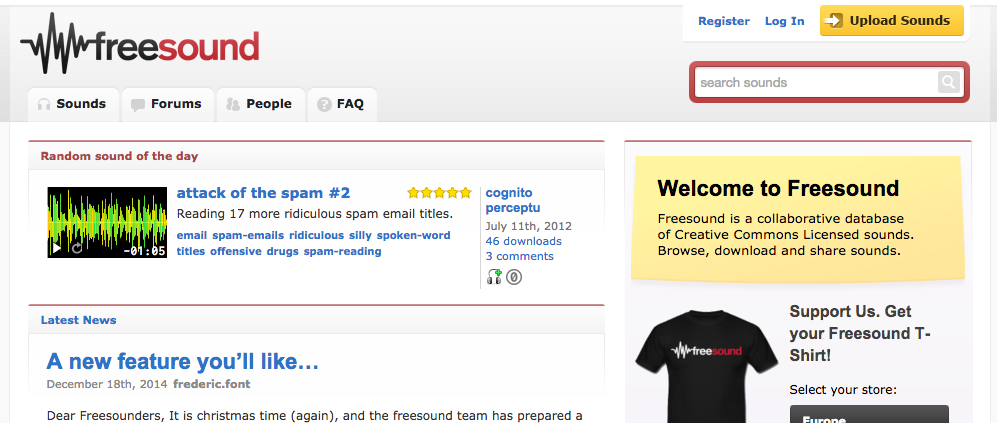
\includegraphics[width=\textwidth]{freesound.png}
\caption{Screenshot of the Freesound.org homepage. Immediately visible are both the semantic descriptors ascribed to a particular sound (left), and the primary search mechanism, a text field (right).}
\label{fig:freesound}
\end{figure}

% Representation for efficient search and retrieval; approximate nearest neighbors, LSH
The development of a robust timbre space would not only make it possible to search for sounds with sounds, bypassing the linguistic intermediary, but also facilitate the ranking of potentially relevant results by providing a notion of distance.
% User interfaces and visualization
This concept of a metric timbre space is also particularly attractive in the realm of user interfaces and visualization.
Euclidean spaces are easily relatable by physical analogy, and visualization allows for acoustic information to be understood in an intuitive manner.
% Artistic Exploration and Composition
The ability to explore familiar ideas from an unfamiliar perspective holds considerable merit for artistic exploration and new approaches to composition.
% TODO: Juan says weak; I don't disagree, just not sure that I care.


\subsection{Limitations}

It is valuable to note that despite the difficulty inherent to defining timbre, all computational research must adopt some working concept of it, implicitly or otherwise.
Generally two facets to timbre; sound quality and sound source.
They are related but not exactly equal.
The work presented here operates on the assumption that the perception of timbre is tightly coupled with the experience of discriminating between unique sound sources.
This is not intended to be a true equivalence with timbre, but a functional approximation that allows the research to proceed.
Compromise and simplification; You'll pay out somewhere.
Human judgements of similarity absolve you assumptions about the relationship between source and quality, but costly to curate at scale.
A data-driven approach, on the other hand, offers the opposite scenario; it is relatively simple to collect this data, but requires that assumptions be made regarding the quality being related.

Ensemble versus solo.
Here focus entirely on the latter.




\section{Learning Timbre Similarity}
\label{sec:timbre_similarity}

From the previous review of psychoacoustics research and efforts to computationally explain timbre, there is an important series of observations to consider.
Classic timbre features are discovered through an involved process of designing a number of signal-level statistics and identifying which correlate with the dimensions of a model.
Importantly, those statistics that best explain a timbre space are only valid in the context of the sound sources considered, and thus the process should be repeated for different sonic palettes.
Additionally, the subjective ratings necessary to conduct this kind of research are costly to obtain.
Therefore, taking cues from the discussion of Chapter \ref{chp:context}, these practical challenges encourages the use of feature learning to automate the development of timbre similarity models.

Having discussed the value and applications of computational timbre similarity space, it is worthwhile to outline the goals for such a system.
First and foremost, one would learn, rather than design, signal-level features relevant to achieve the given task and circumvent the issues identified previously.
This idea is based on the combination of an inability to clearly define the sensory phenomenon, while affording the flexibility to change the space of timbres considered.
Additionally, sound should be represented in an intuitive manner, such that distance between points is semantically meaningful.
In other words, signals from the same source should be near-neighbors, whereas sounds from different sources should be far apart.
% Come back to how we show this in the methodology.
Finally, the ideal similarity space is perceptually \emph{smooth}, meaning that a point that interpolates the path between two others should be a blend of the two, e.g. a tenor saxophone might fall between a clarient and a French horn.

These objectives share conceptual overlap with dimensionality reduction methods and instrument classification systems, on which this work builds.
In lieu of precise information regarding the relationship between two given sounds, music instrument classes are used as a proxy for timbre similarity.
The approach presented here consists of four components, as diagrammed in Figure \ref{fig:nlse}, and discussed in the following subsections.
First, all audio is transformed into a time-frequency representation (Subsection \ref{subsec:timbre_tfr}).
The main component of the system is a deep convolutional network, which maps tiles of these time-frequency coefficients into a low-dimensional space (Subsection \ref{subsec:timbre_deepnet}).
A pairwise training harness is made by copying this network, and parameters are learned by minimizing the distance between observations of the same sound source and maximizing the distance otherwise (Subsection \ref{subsec:timbre_pairwise}).
At test time, the pairwise harness is discarded, and the resulting network is used to project inputs to the learned embedding space.


\begin{figure}[t]
\centering
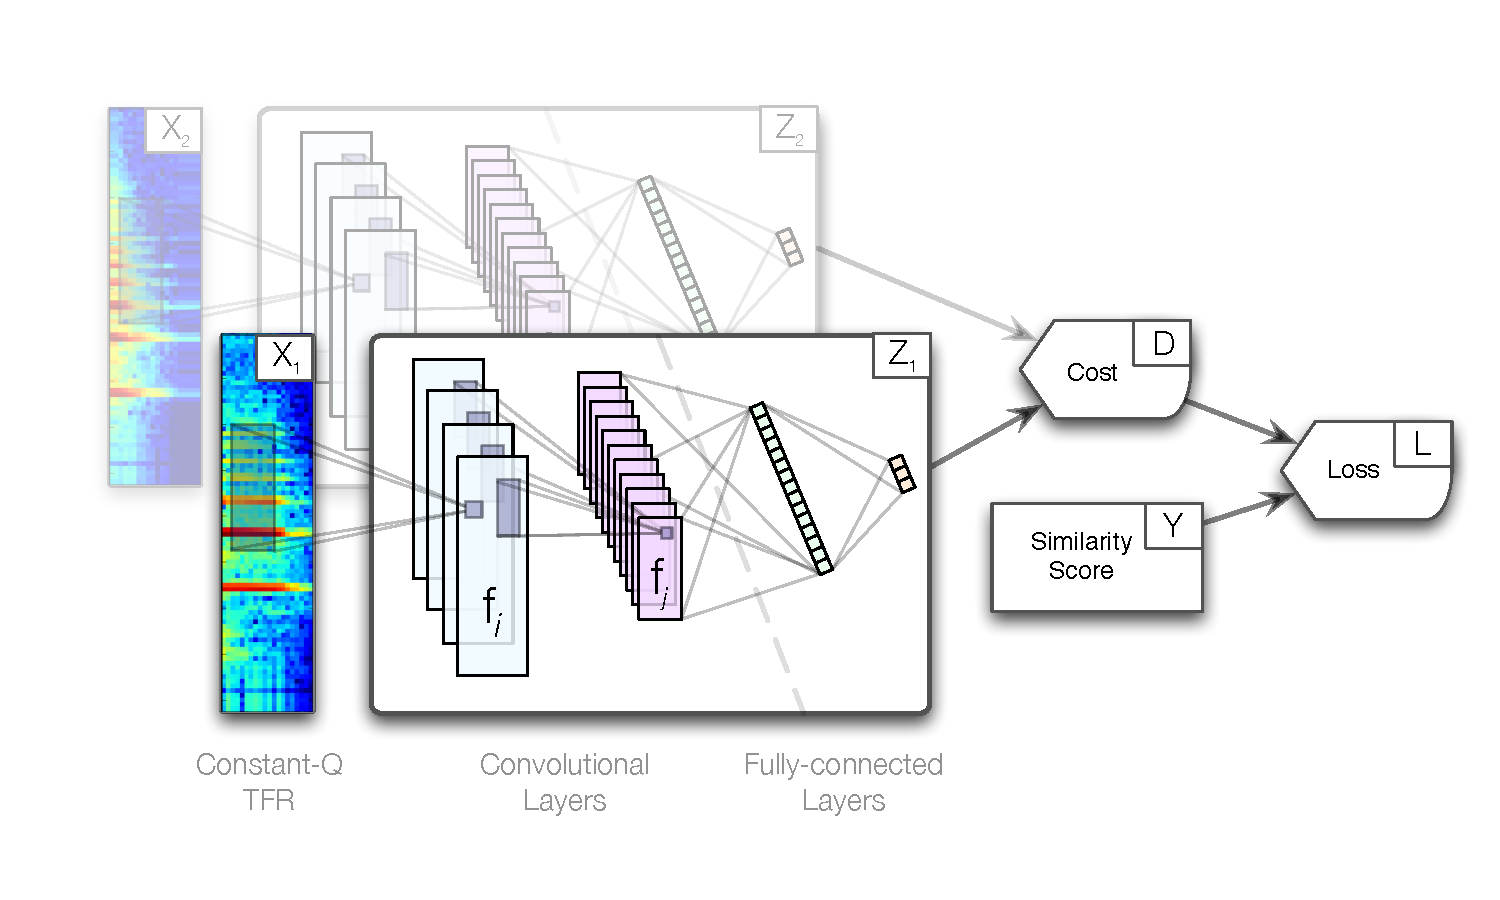
\includegraphics[width=\textwidth]{nlse_system.pdf}
\caption{Diagram of the proposed system: a flexible neural network is trained in a pairwise manner to minimize the distance between similar inputs, and the inverse of dissimilar ones.}
\label{fig:nlse}
\end{figure}


\subsection{Time-Frequency Representation}
\label{subsec:timbre_tfr}

Time-domain audio signals are first processed by a Constant-Q transform (CQT).
The most important benefit of this particular filterbank is that the CQT is logarithmic in frequency.
While this serves as a reasonable approximation of the human auditory system, it has the practical benefit of linearizing convolutions in pitch as well as time.
It is generally agreed upon that timbre perception is, at least to some degree, invariant to pitch, and this allows the network to behave similarly.

The constant-Q filterbank is parameterized as follows: all input audio is first downsampled to 16kHz; bins are spaced at 24 per octave, or quarter-tone resolution, and span eight octaves, from 27.5Hz to 7040Hz; analysis is performed at a framerate of 20Hz uniformly across all frequency bins.
Logarithmic compression is applied to the frequency coefficients with an offset of one, i.e. $log(X + 1.0)$. % TODO: Does this not need scalaing? where $X$ is the input magnitude coefficients and $C$ is some large, positive scalar; here, this value is set to 100.


\subsection{Deep Convolutional Networks for Timbre Embedding}
\label{subsec:timbre_deepnet}

Noting that the details of deep learning and convolutional networks are discussed at length previously, only those decisions unique to this task are addressed here; for clarity regarding the mathematical or conceptual definitions of these terms, refer to Chapter \ref{chp:deep_learning}.

A five-layer neural network is designed to project time-frequency inputs into a low-dimensional embedding.
The first three layers make use of 3D-convolutions, to take advantage of translation invariance, reduce the overall parameter space, and act as a constraint on the learning problem.
Max-pooling is applied in time and frequency, to further accelerate computation by reducing the size of feature maps, and allowing a small degree of scale invariance in both directions.
The final two layers are fully-connected affine transformations, the latter of which yields the embedding space.
The first four hidden layers use a hyperbolic tangent as the activation function, while the visible output layer is linear, i.e. it has no activation function in the conventional sense.

Hyperbolic tangents are chosen as the activation function for the hidden layers purely as a function of numerical stability.
It was empirically observed that randomly initialized networks designed with rectified linear units instead were near impossible to train; perhaps due to the relative nature of the learning problem, i.e. the network must discover an equilibrium for the training data, the parameters were routinely pulled into a space where all activations would go to zero, collapsing the network.
Conversely, hyperbolic tangents, which saturate and are everywhere-differentiable, did not suffer the same fate.
It is possible that the use of activation functions that provide an error signal everywhere, such as sigmoids or ``leaky'' rectified linear units \cite{Maas2014}, or better parameter initialization might avoid this behavior, but neither are explored here.

It was observed in the course of previous research, that the use of a saturating nonlinearity at the output of the embedding function can lead to problematic behavior \cite{Humphrey2011}.
As will be discussed in more detail shortly, bounded outputs makes the choice of hyperparameters crucial in order to prevent the network from pushing datapoints against the limits of its space, and thus the output layer is chosen here to be linear.
The absence of boundaries allows the network to find an appropriate scale factor for the embedding.
This is similar in principle to the practice of linear ``bottleneck'' layers  in other embedding systems \cite{Liao2013}.

% Specifically, the network is parameterized thusly.
The input to the network is a 2D tile of log-CQT coefficients with shape $(20, 192)$, corresponding to time and frequency respectively.
The frequency channels of the CQT span eight octaves, from 27.5 to 7040 Hz, with quarter-tone resolution.
The first convolutional layer uses 20 filters with shape $(1, 5, 13)$ and max-pooling with shape $(2, 2)$.
The max-pooling in time introduces a small degree of temporal scale invariance, while the same operation in frequency serves to reduce quartertone to semitone resolution.
The second convolutional layer uses 40 filters with shape $(20, 5, 11)$ and max-pooling with shape $(2, 2)$, and the third convolutional layer uses 80 filters with shape $(1, 1, 9)$ and max-pooling with shape $(2, 2)$;
in both instances, max-pooling is used to further reduce dimensionality while introducing more scale invariance.
The fourth layer is fully-connected and has 256 output coefficients, while the final layer is also fully connected and has 3 output coefficients.


\subsection{Pairwise Training}
\label{subsec:timbre_pairwise}

% Relative vs absolute
In the absence of this subjective pairwise instrument ratings, instrument taxonomies are used as a proxy for timbre similarity.
This approach to defining timbre ``neighborhoods'' is used to extend the work of Hadsell et al \cite{Hadsell2007} to address this challenge of learning a timbre similarity space.
Referred to by the authors as ``dimensionality reduction by learning an invariant mapping'' (DrLIM), a deep network was trained in a pairwise manner to minimize the distance between ``similar'' data points in a learned, nonlinear embedding space, and vice versa.
Similarity was determined in an unsupervised manner by linking the $k$-nearest neighbors in the input space.
Though left as future work, the authors propose that other information, such as class relationships, might be levereaged to learn different embeddings.
This is an important consideration for the problem of timbre, because fundamental frequency and amplitude are likely to dominate the graph of nearest neighbors defined in the input space alone.

The intution behind DrLIM is both simple and satisfying: datapoints that are deemed ``similar'' should be close together, while those that are ``dissimilar'' should be far apart.
Though the precise distance metric is a flexible design decision, it is used here in the Euclidean sense.
A collection of similar and dissimilar relationships can be understood by analogy to a physical system of attractive and repulsive forces, where learning proceeds by finding a balance between them; and furthermore, this analogy illustrates the need for contrasting forces to achieve equilibrium.

% This first sentence blows, come back to this.
At its core, DrLIM is ultimately a pairwise training strategy.
First, a parameterized, differentiable function, $\mathcal{F}(X | \Theta)$, e.g. a neural network, is designed for a given problem;
in the case of dimensionality reduction, the output will be much smaller than the input, and typically either 2 or 3 for the purposes of visualization.
During training, the function $\mathcal{F}$ is copied and parameters, $\Theta$, \emph{shared} between both> %, such that $\mathcal{F}_1(\dot | \Theta) == \mathcal{F}_2(\dot | \Theta)$.
Two inputs, $X_1$ and $X_2$, are transformed by their respective functions, $\mathcal{F}_1$ and $\mathcal{F}_2$, to produce the outputs, $Z_1$ and $Z_2$.
A metric, e.g. Euclidean, is chosen to compute a distance, $D$ between these outputs.
Finally, a similarity score, $Y$, representing the relationship between $X_1$ and $X_2$, is passed to a contrastive loss function, which penalizes similar and dissimilar pairs differently.
Generalizing the original DrLIM approach, different margin terms are applied in the two conditions.
For similar pairs, the loss will be small when the distance is small, or zero within the margin $m_s$;
for dissimilar pairs, the loss will be small when the distance is large, or zero outside a dissimilar margin, $m_d$.
This formal definition is summarized symbolically by the following:


\begin{align*}
Z_1 = \mathcal{F}_1(X_1 | \Theta), Z_2 = \mathcal{F}_2(X_2 | \Theta)\\
D = || Z_1 - Z_2 ||_2\\
\mathcal{L}_{s} = \max(0, D^2 - m_{s})\\
\mathcal{L}_{d} = \max(0, m_{d} - D)^2\\
\mathcal{L} = Y * \mathcal{L}_{s} + (1 - Y) * \mathcal{L}_{d} \\
\end{align*}

\noindent Note that similarity is given by $Y=1$, for consistency with boolean logic.
As a result, the first term of the loss function is only non-zero for similar pairs, and the inverse is true for the second term.

%Training strategy
Returning to the previous discussion regarding the dynamic range of the output layer, it should now be clear that the choice of margin only influences the learned embedding relative to a scale factor when the output is unbounded.
The two loss terms are mirrored parabolas, and changing the margin, or horizontal offset, only serves to shift the vertical line about which they reflect.
The curvature, and thus the gradient, of the loss function is left unchanged.
% This observation encourages a simple generalization of this loss function, where a second margin is introduced to the ``similar'' loss term:

% \begin{align*}
% \mathcal{L}_{sim} = max(0, D - m_{sim})^2\\
% \mathcal{L}_{diff} = max(0, m_{diff} - D)^2\\
% \mathcal{L} = Y * \mathcal{L}_{sim} + (1 - Y) * \mathcal{L}_{diff} \\
% \end{align*}

% This generalized square-square loss is shown in Figure \ref{fig:double_margin} for various margin values.
Whereas the differential margin controls the spread of all points in space, the similar margin will control the spread of a similarity neighborhood.
In the original formulation, where implicitly $m_{sim} = 0$, the loss is lowest when all inputs are mapped to \emph{exactly} the same point; for the purposes of similarity, a more diffuse distribution of points is desirable.
It is worth noting the slight parallel to linear discriminant analysis, a statistical method that seeks to jointly minimize intraclass variance and maximize interclass variance.
Given the relative nature of this trade-off, it is sufficient to pick a single ratio between the margins, eliminating the need to vary both hyperparameters separately.


In practice, training proceeded via minibatch stochastic gradient descent with a constant learning rate, set at 0.02 for 25k iterations, or until a batch returned a total loss of zero.
Batches consisted of 100 comparisons, drawn such that a datapoint was paired with both a positive and negative example.


\section{Methodology}
\label{sec:methodology}

% Here's the explanation of what was done.
% What are the questions we want to address?

To assess the viability of data-driven nonlinear semantic embeddings for timbre similarity, and thus address the goals outlined at the outset of Section \ref{sec:timbre_similarity}, two experiments are used to quantify different performance criteria.
First, the local structure and class boundaries of the learned embeddings are explored with a classification task.
Second, global organization of the space is measured by a ranked retrieval task.
Additionally, in lieu of a subjective evaluation of perceptual ``smoothness'' of the resulting timbre space, the learned embeddings are investigated through confusion analysis and visualization.
In each instance, the approach presented here is compared to a conceptually similar, albeit admittedly simpler, system.

Finally, the formulation described in the previous section presents two system variables, thus giving rise to two additional considerations:

\begin{enumerate}
\item What is the effect of using different margin ratios?
\item How does the sonic palette considered impact the learned embedding?
\end{enumerate}


\subsection{Data}
The data source used herein is drawn from the Vienna Symphonic Library (VSL), a truly massive collection of studio-grade orchestral instrument samples recorded over a variety of performance techniques\footnote{\url{https://vsl.co.at/en}}.
In aggregate, the VSL contains over 400k sound recordings from more than 40 different instruments, both pitched and percussive.
Sorting instrument classes by sample count yields 27 instruments with at least 5k samples; three of these instruments, however, are not reasonably distinct from other sources, e.g. ``flute-1'' and ``flute-2'', and discarded rather than risk introducing conflicting information.
This decision yields the set of instruments contained in Table \ref{tab:all_insts} for experimentation.


\begin{table*}[t]
\begin{center}
\caption{Instruments considered and their corresponding codes.}
\begin{tabular}{l | c || l | c}
Instrument & Code & Instrument & Code \\
\hline
French Horn & ho & Tuba & tu\\
Violin & vi & Cimbasso & ci \\
B$\flat$ Clarinet & klb & Piccolo & pt \\
Tenor Trombone & tp & Oboe & ob \\
C Trumpet & trc & Bass Clarinet & bkl \\
Bass Trombone & bp & Wagner Tuba & wt \\
Acoustic Concert Guitar & akg & Contra Bassoon & kfa \\
Bassoon & fa & English Horn & eh \\
Cello & vc & Bass & kb \\
Bass Trumpet & bt & Soprano Saxophone & sxs \\
Distorted Guitar & eg & Tenor Saxophone & sxt \\
Flute & fl & Alto Flute & afl \\
\hline
\end{tabular}
\label{tab:all_insts}
\end{center}
\end{table*}


The distribution of sound files for these instruments, grouped by class, is given in Figure \ref{fig:c24_dist}.
As discussed previously, it is an inherent difficulty of pairwise similarity models that the resulting relationships are limited by the number of unique classes considered.
Fortunately, there is no added cost to considering a wider palette of sound sources here because the label information is objective.
Therefore, building upon previous work \cite{Humphrey2011}, three configuration subsets are repeated from the pilot study as well as a fourth consisting of all 24 classes, given in Table \ref{tab:palette}.

\begin{figure}[t]
\centering
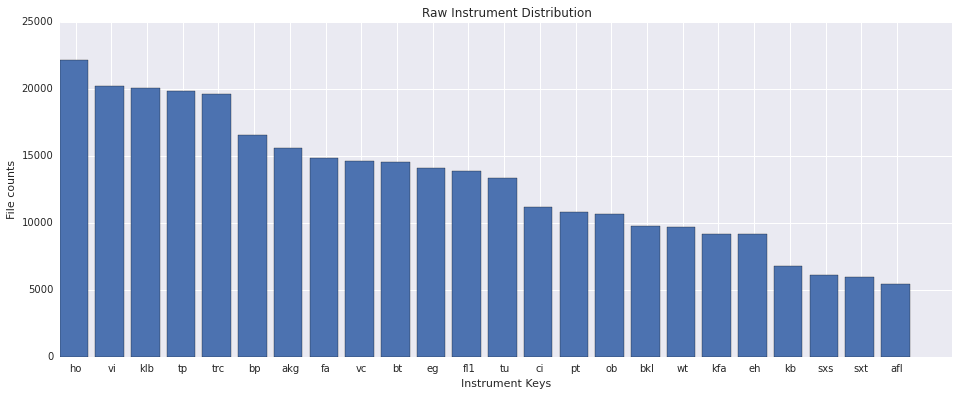
\includegraphics[width=\textwidth]{raw_vsl_distribution.png}
\caption{Distribution of instrument samples in the Vienna Symphonic Library.}
\label{fig:c24_dist}
\end{figure}


\begin{table*}[t]
\begin{center}
\caption{Instrument set configurations.}
\begin{tabular}{l | l }
Key & Instrument Codes \\
\hline
c5 & tu, ob, klb, vc, fl \\
c8 & trc, ho, ob, eh, klb, sxt, vi, vc \\
c12 & c8 + \{tp, tu, fa, fl\} \\
c24 & c12 + \{bp, akg, bt, eg, ci, pt, bkl, wt, kfa, kb, sxs, afl\} \\
\hline
\end{tabular}
\label{tab:palette}
\end{center}
\end{table*}

For each instrument class, 5k samples are drawn, without replacement, to build a uniformly distributed collection.
This step simplifies the process of data sampling during stochastic training of the network, which may be sensitive to class imbalances.
The collection of instrument samples is stratified into five equal partitions for cross validation, used at a ratio of 3-1-1 for training, validation, and testing, respectively.
The partitions are circularly rotated such that each is used as the test set once, i.e. (1, 2, 3)-4-5, (2, 3, 4)-5-1, and so on.


\subsection{Margin Ratios}

Though the pairwise training strategy described in Section \ref{subsec:timbre_pairwise} consists of two margin hyperparameters, it is ultimately the ratio between the two that governs how the space will be shaped.
In isolation, the exact choice of dissimilar term's margin, $m_{d}$, is inconsequential and determines the radius of the bounding sphere.
Going forward, this value is fixed to $\sqrt{12}$, corresponding to the radius of the sphere that intersects the coordinate $(2, 2, 2)$.
Moving the similar term's margin, $m_{s}$, relative to this value will lead to different embeddings, and three ratios of $m_{s}:m_{d}$ are considered here: 0, $\frac{1}{4}$, and $\frac{1}{2}$.
The corresponding loss functions are shown in Figure \ref{fig:margins}.


\begin{figure}[h]
\centering
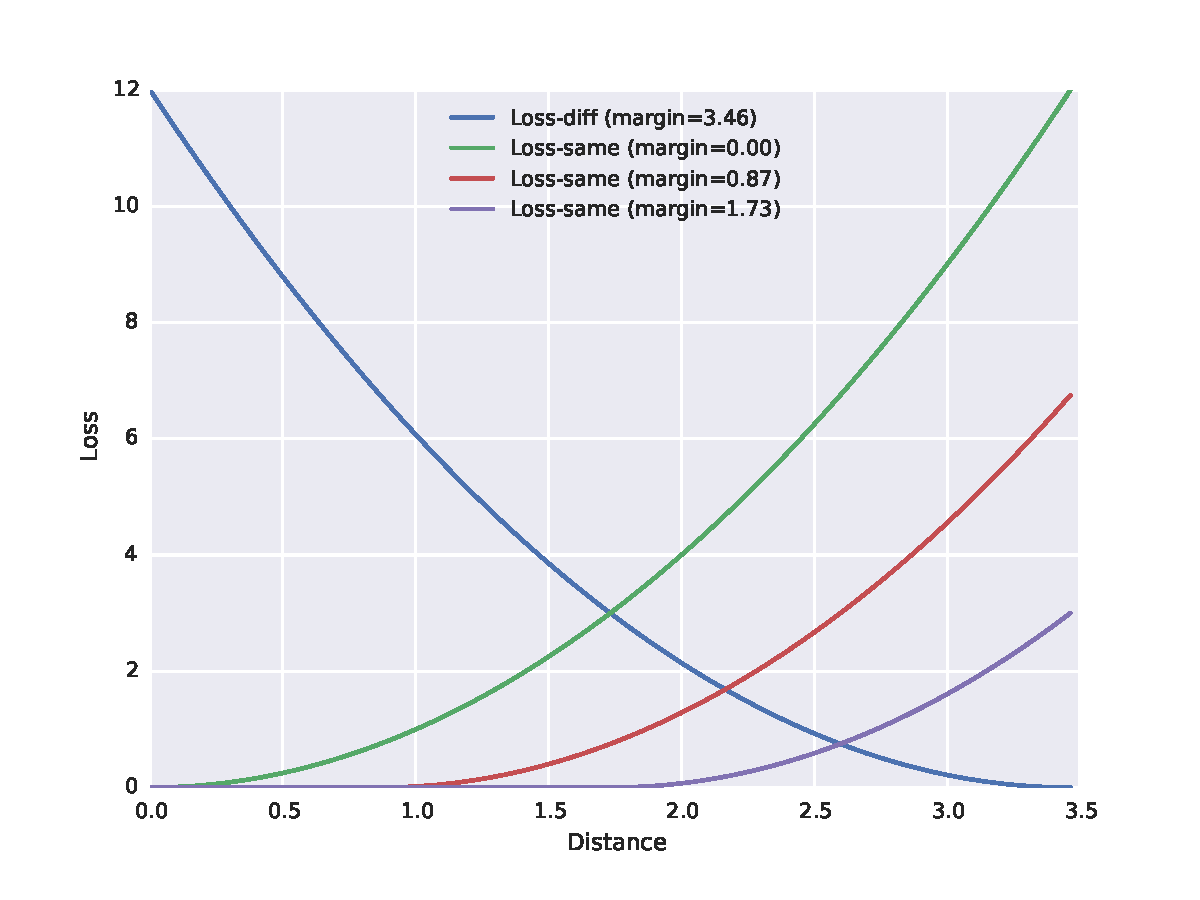
\includegraphics[width=\textwidth]{loss_margins.pdf}
\caption{Loss contours for different margin ratios.}
\label{fig:margins}
\end{figure}



\subsection{Comparison Algorithm}

For the purposes of comparison, a similarly motivated system is constructed using the combination of principal components analysis (PCA) and linear discriminant analysis (LDA).
Previous work explored the application of PCA alone and locally linear embedding as alternative approaches to dimensionality reduction.
Both are unsupervised methods, and do not make for the most fair comparison against a supervised neural network.
LDA, however, is a supervised approach to dimensionality reduction, and shares at least a conceptual parallel to the proposed system, as mentioned briefly in Section \ref{subsec:timbre_pairwise}.

It is important to note though that LDA can exhibit odd behavior in high dimensional spaces, and projecting into a PCA subspace first can help alleviate these issues \cite{PCASubspace?}.
This subspace projection is further motivated by computational efficiency concerns, where the input dimensionality is prohibitive to training.
Additionally, the cascade of PCA followed by LDA mimics a two-layer neural network, and is interchangable with the framework described here.
Using the same input dimensions, $20\times192$, a whitened PCA transform is fit to a large sample of the training set.
The principal 256 components are preserved, based on an empirical exploration of the explained variance as well as a midway point in the dimensionality reduction of the system, i.e. the number of cofficients decreases near-equally between the PCA and LDA stages.
After applying the PCA transform to the training sample, an LDA transform is fit to the same data and its corresponding instrument classes, yielding a 3-dimensional embedding.


\subsection{Experimental Results}

As an initial quantitative inquiry, trained models are tested on a classification task using the k-Nearest Neighbors classifier in scikit-learn\footnote{\url{http://scikit-learn.org/stable/}}.
First, networks are trained across the 4 instrument configurations, 3 margin ratios, and 5 folds, and all data are projected into the resulting embedding space.
From here, a collection of points are sampled from each parition --50k, 10k, 25k-- for training, validation, and test, respectively.
The training set is used to fit the classifier, while the validation set is used to identify an optimal setting for the parameter $k$, corresponding to the number of neighbors considered in the decision rule.
Classification accuracy is then computed across all three sets, and tallied across folds to produce averages and standard deviations across the various conditions; these results are given in Tables \ref{tab:train}-\ref{tab:test}.


%train
\begin{table*}[h!]
\begin{center}
\caption{kNN classification results over the training set.}
\small
\begin{tabular}{lllll}
 config  & c5    & c8   & c12  & c24  \\
\hline
 NLSE : 0.0  & $93.81\pm0.53$ & $89.97\pm0.40$ & $86.70\pm0.39$ & $74.17\pm0.79$ \\
 NLSE : 0.25 & $94.21\pm0.18$ & $90.25\pm0.54$ & $87.17\pm0.35$ & $73.91\pm0.61$ \\
 NLSE : 0.5  & $93.04\pm0.29$ & $89.16\pm0.27$ & $86.08\pm0.26$ & $71.59\pm0.88$ \\
 \hline
 PCA-LDA & $64.44\pm0.47$ & $56.58\pm0.60$ & $47.22\pm0.45$ & $35.81\pm0.28$ \\

\hline
\end{tabular}
\label{tab:train}
\end{center}
\end{table*}

\begin{table*}[h!]
\begin{center}
\caption{kNN classification results over the validation set.}
\small
\begin{tabular}{lllll}
\hline
config & c5  & c8 & c12   & c24     \\
\hline
 NLSE, $\frac{m_s}{m_d}=0.0$  & $92.37\pm0.64$ & $87.94\pm0.45$ & $84.52\pm0.97$ & $70.86\pm1.51$ \\
 NLSE, $\frac{m_s}{m_d}=0.25$ & $93.75\pm0.53$ & $88.62\pm0.58$ & $85.65\pm0.26$ & $71.46\pm0.63$ \\
 NLSE, $\frac{m_s}{m_d}=0.5$  & $91.75\pm0.67$ & $87.78\pm0.85$ & $83.78\pm0.53$ & $66.37\pm1.69$ \\
 \hline
 PCA-LDA & $59.97\pm0.96$ & $52.49\pm2.68$ & $39.25\pm2.01$ & $24.32\pm0.97$ \\
\hline
\end{tabular}
\label{tab:valid}
\end{center}
\end{table*}

\begin{table*}[h!]
\begin{center}
\caption{k-Neighbors classification results over the testing set.}
\small
\begin{tabular}{rllll}
\hline
config & c5  & c8  & c12   & c24   \\
\hline
 NLSE, $\frac{m_s}{m_d}=0.0$  & $92.49\pm0.41$ & $88.26\pm0.74$ & $84.35\pm0.41$ & $70.67\pm0.55$ \\
 NLSE, $\frac{m_s}{m_d}=0.25$ & $92.97\pm0.41$ & $88.67\pm0.79$ & $85.16\pm0.24$ & $70.28\pm0.86$ \\
 NLSE, $\frac{m_s}{m_d}=0.5$  & $91.96\pm0.35$ & $87.83\pm0.25$ & $84.04\pm0.57$ & $66.91\pm0.57$ \\
 \hline
 PCA-LDA  & $59.91\pm0.77$ & $50.24\pm1.52$ & $39.32\pm0.86$ & $24.77\pm0.51$ \\
\hline
\end{tabular}
\label{tab:test}
\end{center}
\end{table*}


A few conclusions are immediately obvious from these results.
Most striking is the performance discrepancy between the NLSE and the PCA-LDA models.
Previous work demonstrated a significant margin between the unsupervised dimensionality reduction methods, and this result shows that the difference is indeed a function of complexity, not just the supervised learning process.
To a lesser extent, all models show some degree of over-fitting, but the effect is more severe for the PCA-LDA model than any NLSE.
It is interesting to note that a non-zero similarity margin, $m_s$, leads to slightly better classification results than the centered loss function.
One explanation for such behavior is that introducing a small region of zero-loss within a class may allow the network to emphasize dissimilar relationships more as training proceeds.
It would appear too much freedom, on the other hand, leads to fuzzy boundaries between classes and begins to compromise local structure.


The outcome of the classification experiment can also be used to inform how smooth or intuitive this space might be.
To do so, confusion matrices are shown for the c12 configuration for the best NLSE, with a margin ratio of 0.25, and the PCA-LDA model, in Tables \ref{tab:confmat_nlse} and \ref{tab:confmat_pcalda}, respectively.


% \begin{table*}[h]
% \begin{center}
% \caption{Confusion Matrix -- (c12, ratio=0.0).}
% \scriptsize
% \begin{tabular}{ccccccccccccc}
% \hline
%    & eh &    fa &   fl &    ho &   klb &    ob &   sxt &    tp &   trc &    tu &    vc &    vi \\
% \hline
% eh &  \textbf{84.96} &  0.65 &  0.76 &  1.41 &  1.43 &  5.73 &  1.52 &  0.33 &  2.60 &  0.22 &  0.47 &  1.09 \\
% fa &   1.65 & \textbf{84.30} &  0.08 &  3.98 &  0.25 &  0.37 &  1.19 &  0.90 &  0.95 &  4.04 &  2.31 &  0.54 \\
% fl &   0.88 &  0.17 & \textbf{85.42} &  0.71 &  2.56 &  3.65 &  3.24 &  0.13 &  1.57 &  0.23 &  0.51 &  0.75 \\
% ho &   0.93 &  2.21 &  0.10 & \textbf{80.74} &  0.20 &  0.30 &  0.79 &  9.28 &  2.59 &  3.57 &  0.53 &  0.65 \\
% klb &   1.02 &  0.12 &  1.52 &  0.64 & \textbf{85.38} &  4.93 &  3.46 &  0.12 &  1.01 &  0.31 &  2.30 &  0.54 \\
% ob &   2.67 &  0.16 &  2.92 &  0.87 &  1.74 & \textbf{83.02} &  0.63 &  0.12 &  4.06 &  0.16 &  0.16 &  1.33 \\
% sxt &   0.29 &  0.36 &  0.80 &  0.37 &  1.56 &  0.34 & \textbf{85.60} &  0.10 &  0.94 &  1.37 &  4.70 &  2.27 \\
% tp &   0.51 &  0.45 &  0.06 & 10.97 &  0.06 &  0.34 &  0.46 & \textbf{78.47} &  2.73 &  2.79 &  0.54 &  0.45 \\
% trc &   1.54 &  0.07 &  1.11 &  2.63 &  0.51 &  4.60 &  1.37 &  3.33 & \textbf{83.58} &  0.43 &  0.33 &  1.57 \\
% tu &   0.19 &  2.31 &  0.05 &  4.02 &  0.13 &  0.11 &  1.51 &  2.36 &  0.56 & \textbf{84.69} &  3.27 &  0.32 \\
% vc &   0.44 &  0.50 &  0.19 &  0.50 &  0.84 &  0.29 &  3.46 &  0.17 &  0.43 &  2.23 & \textbf{90.56} &  0.70 \\
% vi &   0.81 &  0.31 &  0.65 &  1.48 &  0.43 &  1.59 &  5.06 &  0.56 &  2.17 &  0.51 &  1.97 & \textbf{85.23} \\
% \hline
% \end{tabular}
% \label{tab:things}
% \end{center}
% \end{table*}

% TODO: Label rows and columns as reference vs estimated.
\begin{landscape}
\begin{table*} % [h]
\begin{center}
\caption{Confusion Matrix for c12; NLSE with a margin ratio of 0.25.}
% \Small
\begin{tabular}{c | cccccccccccc}
\hline      % Actual columns, Predicted rows
   & eh &    fa &   fl &    ho &   klb &    ob &   sxt &    tp &   trc &    tu &    vc &    vi \\
\hline
eh & \textbf{85.52} &  1.10 &  0.46 &  3.05 &  1.76 &  3.05 &  0.44 &  0.23 &  2.53 &  0.30 &  0.51 &  1.64 \\
fa &   1.74 & \textbf{85.82} &  0.05 &  3.93 &  0.26 &  0.19 &  0.63 &  0.81 &  0.51 &  3.64 &  2.48 &  0.51 \\
fl &   0.80 &  0.10 & \textbf{85.20} &  0.90 &  2.19 &  6.00 &  1.67 &  0.14 &  2.33 &  0.07 &  0.33 &  1.17 \\
ho &   0.76 &  1.88 &  0.07 & \textbf{82.52} &  0.26 &  0.29 &  0.33 &  6.50 &  1.18 &  2.73 &  0.88 &  1.26 \\
klb &   1.23 &  0.40 &  2.46 &  1.16 & \textbf{86.57} &  3.02 &  1.80 &  0.11 &  1.01 &  0.25 &  1.37 &  1.05 \\
ob &   2.90 &  0.06 &  3.09 &  1.12 &  2.56 & \textbf{81.22} &  0.44 &  0.17 &  5.29 &  0.04 &  0.04 &  1.39 \\
sxt &   0.24 &  0.38 &  1.01 &  0.51 &  1.24 &  0.84 & \textbf{86.34} &  0.14 &  0.48 &  0.65 &  4.97 &  2.78 \\
tp &   0.39 &  0.87 &  0.10 & 11.87 &  0.03 &  0.49 &  0.20 & \textbf{80.96} &  2.38 &  2.73 &  0.95 &  0.59 \\
trc &   1.14 &  0.11 &  1.77 &  3.84 &  0.56 &  4.13 &  0.59 &  1.74 & \textbf{83.45} &  0.08 &  0.09 &  2.47 \\
tu &   0.04 &  1.55 &  0.04 &  5.32 &  0.04 &  0.01 &  0.57 &  2.18 &  0.09 & \textbf{86.44} &  2.82 &  0.57 \\
vc &   0.27 &  0.53 &  0.24 &  1.51 &  0.79 &  0.49 &  2.68 &  0.27 &  0.63 &  2.32 & \textbf{89.74} &  1.49 \\
vi &   0.49 &  0.23 &  0.61 &  2.44 &  0.46 &  1.20 &  2.46 &  0.48 &  2.05 &  0.41 &  2.06 & \textbf{87.32} \\
\hline
\end{tabular}
\label{tab:confmat_nlse}
\end{center}
\end{table*}
\end{landscape}

% \begin{table*}[h]
% \begin{center}
% \caption{Confusion Matrix -- (c12, ratio=0.5).}
% \scriptsize
% \begin{tabular}{ccccccccccccc}
% \hline
%   &  eh &    fa &   fl &    ho &   klb &    ob &   sxt &    tp &   trc &    tu &    vc &    vi \\
% \hline
%  eh & \textbf{83.85} &  1.13 &  0.56 &  2.70 &  2.05 &  3.89 &  0.67 &  0.27 &  2.35 &  0.20 &  0.78 &  1.55 \\
%  fa &  1.59 & \textbf{83.41} &  0.03 &  5.87 &  0.36 &  0.07 &  0.51 &  0.50 &  0.69 &  3.26 &  2.86 &  0.40 \\
%  fl & 1.15 &  0.04 & \textbf{85.36} &  0.80 &  2.29 &  3.56 &  2.60 &  0.07 &  2.79 &  0.05 &  0.69 &  1.47 \\
%  ho &  0.72 &  1.87 &  0.05 & \textbf{82.06} &  0.26 &  0.24 &  0.25 &  6.52 &  1.17 &  3.54 &  0.85 &  1.42 \\
%  klb &  1.91 &  0.45 &  2.53 &  1.30 & \textbf{84.78} &  3.35 &  2.15 &  0.13 &  1.15 &  0.15 &  1.97 &  1.16 \\
%  ob &  2.88 &  0.05 &  3.38 &  1.05 &  2.73 & \textbf{80.34} &  0.87 &  0.23 &  5.53 &  0.07 &  0.05 &  2.04 \\
%  sxt &  0.21 &  0.42 &  1.45 &  0.34 &  1.18 &  0.53 & \textbf{86.67} &  0.09 &  0.41 &  0.28 &  4.68 &  2.96 \\
%  tp &  0.20 &  0.82 &  0.04 & 14.09 &  0.03 &  0.04 &  0.37 & \textbf{78.79} &  3.38 &  3.30 &  0.66 &  0.96 \\
%  trc &  1.50 &  0.10 &  1.49 &  3.31 &  0.54 &  5.81 &  0.77 &  2.25 & \textbf{82.08} &  0.18 &  0.13 &  2.39 \\
%  tu &  0.13 &  1.97 &  0.01 &  6.18 &  0.04 &  0.00 &  0.45 &  2.31 &  0.22 & \textbf{85.96} &  2.52 &  0.34 \\
%  vc &  0.37 &  0.81 &  0.14 &  1.65 &  0.62 &  0.07 &  2.53 &  0.27 &  0.23 &  1.59 & \textbf{90.40} &  1.61 \\
%  vi &  0.59 &  0.33 &  0.86 &  2.21 &  0.83 &  0.81 &  3.28 &  0.37 &  2.09 &  0.48 &  1.92 & \textbf{85.40} \\
% \hline
% \end{tabular}
% \label{tab:things}
% \end{center}
% \end{table*}

\begin{landscape}
\begin{table*} %[h]
\begin{center}
\caption{Confusion Matrix for c12; PCA-LDA.}
% \Small
\begin{tabular}{c | cccccccccccc}
\hline
     &    eh &    fa &   fl &    ho &   klb &    ob &   sxt &    tp &   trc &    tu &    vc &    vi \\
\hline
 eh  & \textbf{46.10} &  3.01 & 11.27 &  6.79 &  2.61 & 10.92 &  0.21 &  9.69 &  9.85 &  0.79 &  1.20 &  1.04 \\
 fa  &  5.12 & \textbf{46.84} &  0.37 & 14.42 &  0.31 &  0.27 &  1.88 &  7.55 &  0.58 & 17.15 &  2.47 &  0.57 \\
 fl & 13.33 &  1.62 & \textbf{20.82} &  6.93 &  4.01 & 17.74 &  1.79 &  4.26 & 16.32 &  1.63 &  2.10 &  1.85 \\
 ho  &  5.45 & 19.49 &  2.11 & \textbf{43.53} &  1.77 &  0.29 &  0.94 & 15.47 &  1.38 &  7.51 &  1.53 &  4.70 \\
 klb & 10.80 &  4.88 & 11.69 & 10.62 &  \textbf{9.04} &  9.61 &  4.84 &  5.47 & 11.99 &  6.51 &  7.96 &  5.07 \\
 ob  & 15.45 &  0.40 & 17.80 &  1.67 &  3.09 & \textbf{31.93} &  0.56 &  2.42 & 19.92 &  0.69 &  0.81 &  2.14 \\
 sxt &  0.48 &  2.77 &  2.28 &  3.62 &  2.33 &  0.97 & \textbf{47.47} &  1.40 &  3.45 &  9.48 & 14.48 & 15.77 \\
 tp  & 15.98 &  9.58 &  6.45 & 19.43 &  2.02 &  5.74 &  0.52 & \textbf{18.93} &  9.42 &  4.33 &  1.15 &  2.07 \\
 trc & 10.72 &  0.20 & 14.14 &  3.64 &  3.50 & 19.71 &  0.77 &  5.67 & \textbf{36.01} &  0.27 &  1.12 &  4.97 \\
 tu  &  0.04 & 12.39 &  0.06 &  7.13 &  0.77 &  0.03 &  4.35 &  3.68 &  0.03 & \textbf{62.74} &  7.67 &  0.26 \\
 vc  &  0.39 &  1.65 &  2.87 &  2.66 &  2.09 &  2.36 & 18.99 &  1.16 &  4.29 & 10.02 & \textbf{44.95} & 12.05 \\
 vi  &  0.93 &  1.78 &  2.63 &  5.04 &  1.62 &  3.22 & 13.43 &  1.44 &  7.86 &  1.43 &  4.49 & \textbf{56.47} \\
\hline
\end{tabular}
\label{tab:confmat_pcalda}
\end{center}
\end{table*}
\end{landscape}

Though more confusions are to be expected in the PCA-LDA model, given the classification accuracy, it is important to note that these errors are distributed somewhat uniformly across classes, rather than correlated with instrument similarity.
This higher noise-floor indicates that the instruments' distribution exhibit a good deal of overlap in space.
Some logical confusions seem unavoidable, such as french horn (ho) and trombone (tp), or flute (fl) and oboe (ob), occuring in both models.
The former makes sense given common instrument families, i.e. brass, while the latter likely arises from the upper range of the instruments, which has fewer harmonics.


Other instrument relationships also appear to confound some element of pitch height in similarity, particularly for the PCA-LDA model.
This is observed in the confusions between tuba, bassoon, and French horn.
In the NLSE model, tuba is confused with French horn more often than bassoon; for the PCA-LDA model, however, the inverse is true.
Intutively, the two brass instruments should share the higher confusion rate, and thus pitch is being used by the LDA model as a feature with which to distinguish between classes.
The convolutional model, on the other hand, is forced to embrace a considerable amount of pitch invariance, and is prevented from making the same error.

\begin{figure}[h]
\centering
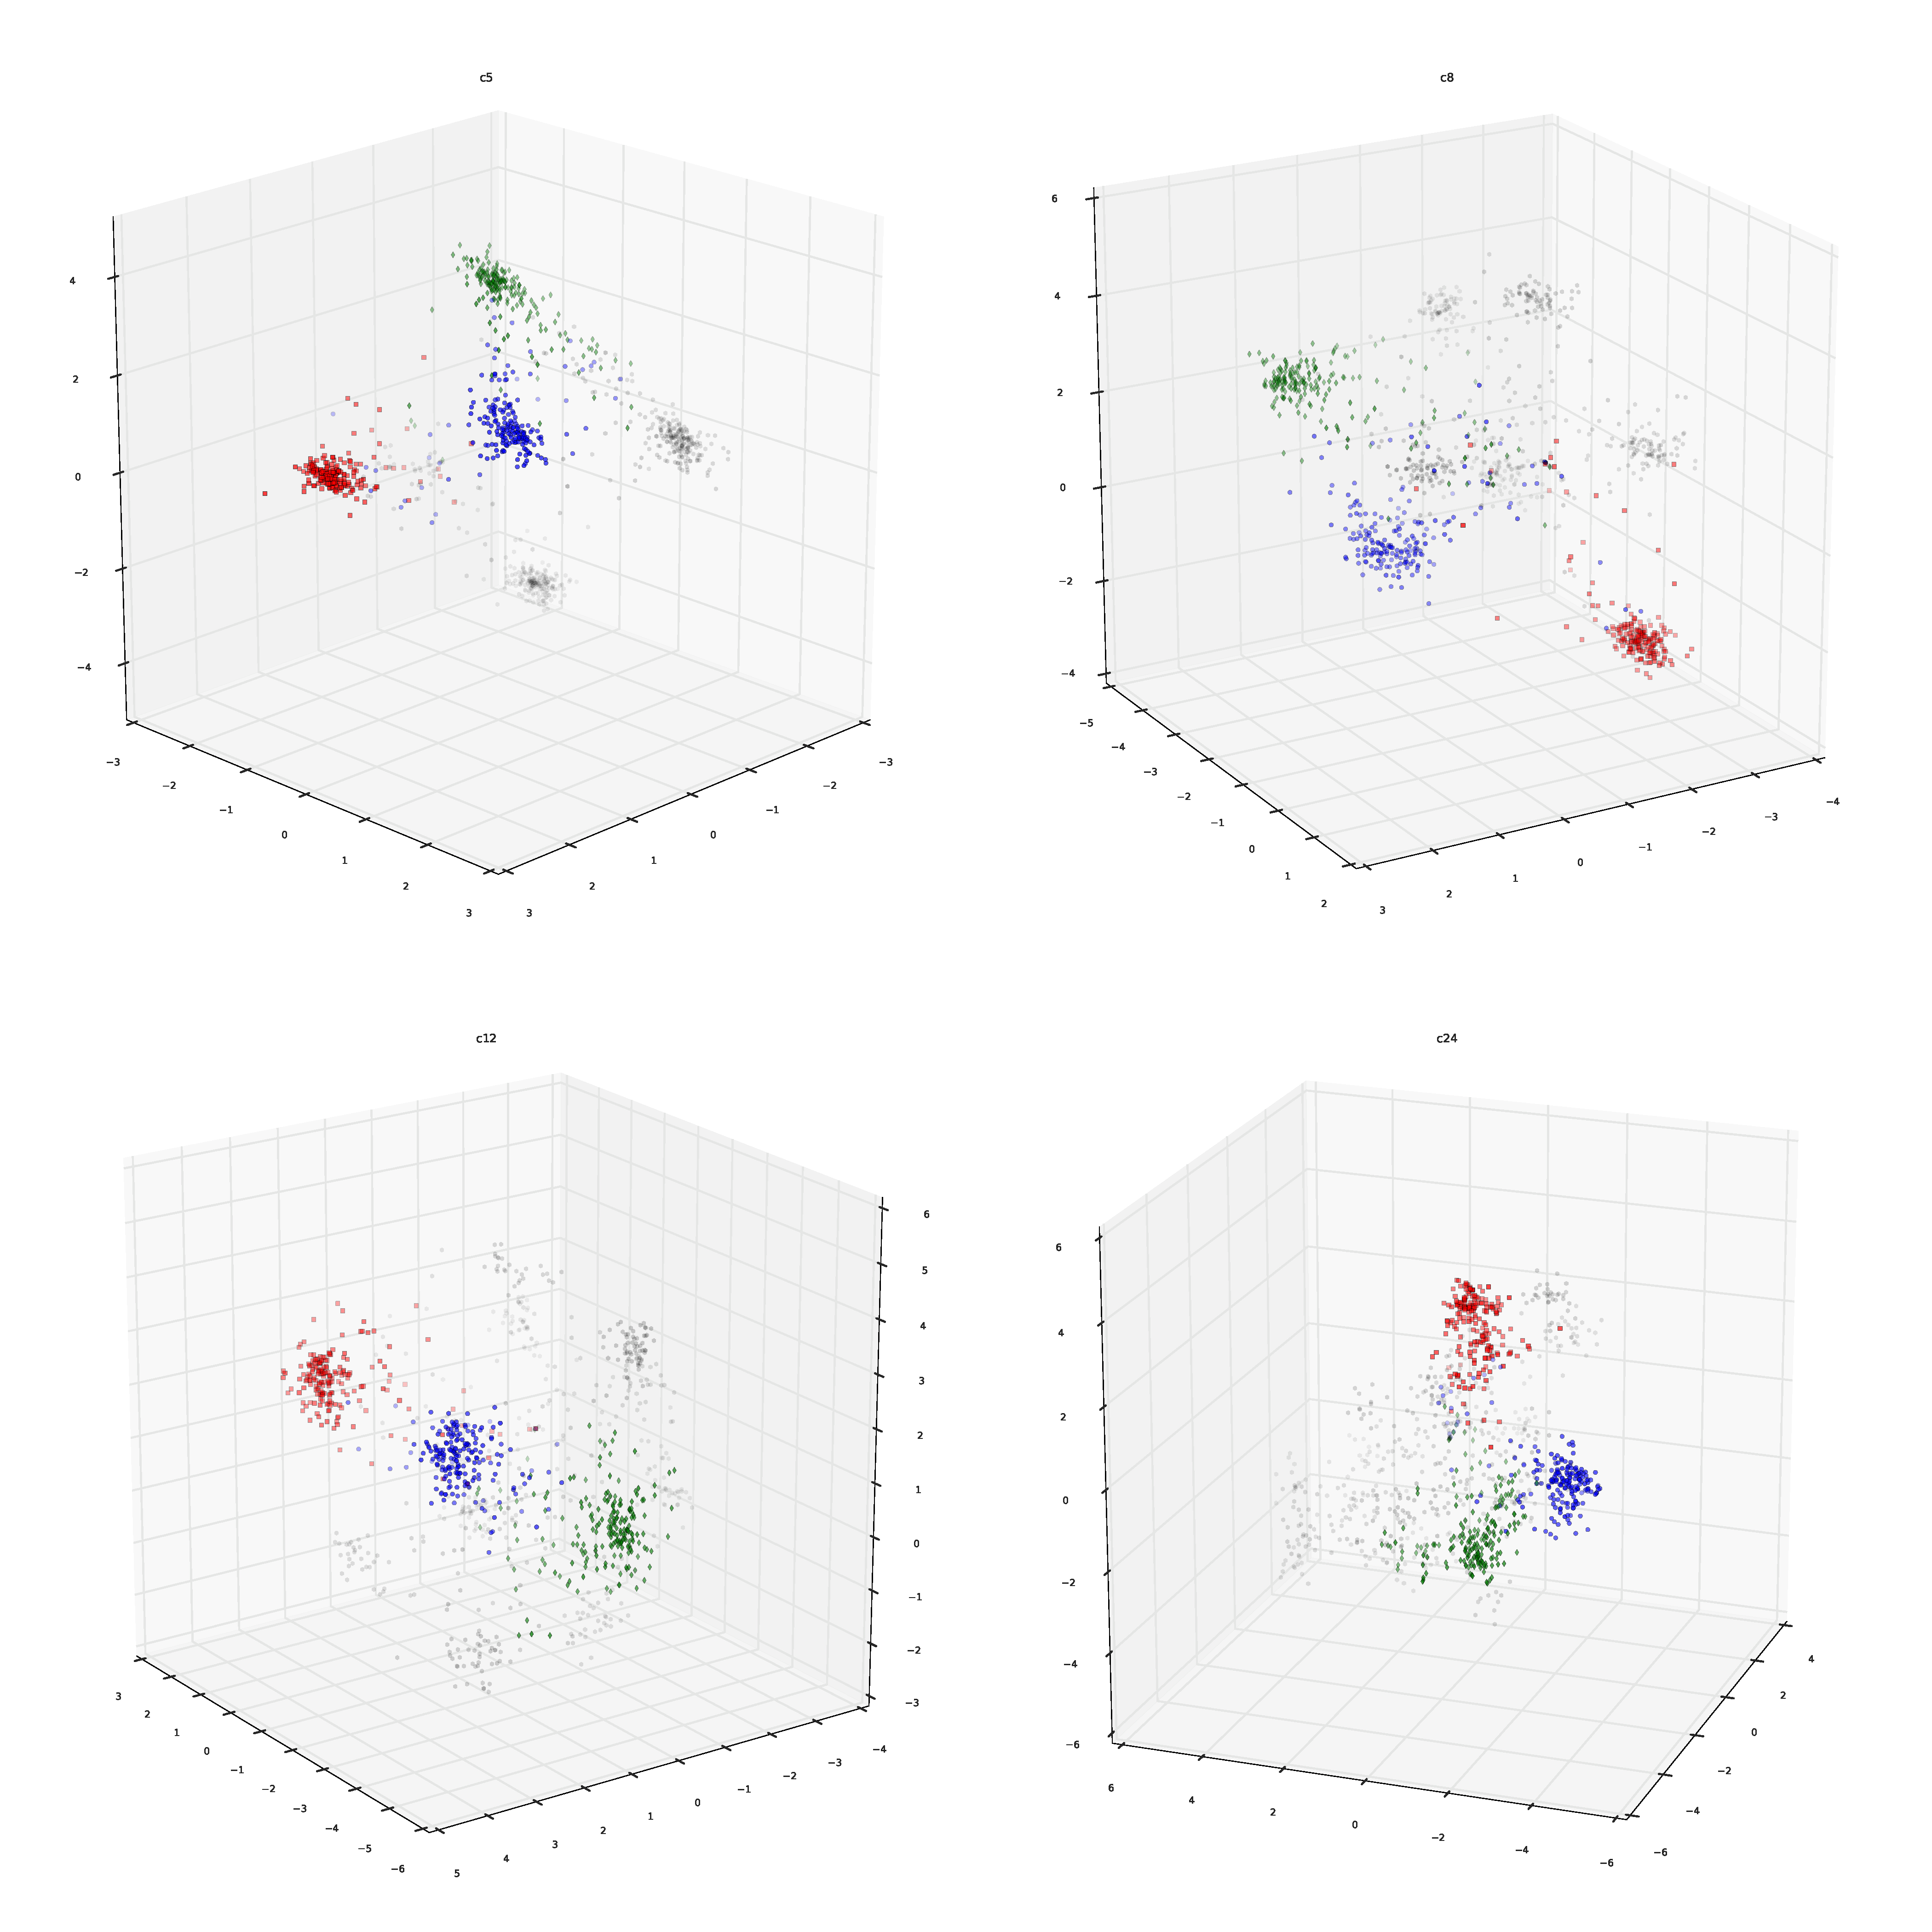
\includegraphics[width=\textwidth]{embeddings_0x25.pdf}
\caption{Embeddings of clarinet (blue circles), oboe (green diamonds), and cello (red squares) observations across models trained with the four different instrument configurations.}
\label{fig:embeddings_0x25}
\end{figure}

To help illustrate the semantic organization of the learned embedding, 3D scatter plots are given in Figure \ref{fig:embeddings_0x25} following observations of the three instruments common to all configurations --clarinet, oboe, cello-- across the different embeddings for $\frac{m_s}{m_d} = 0.25$.
Other instruments are displayed as semi-transparent black to help highlight the three instruments of interest, while giving an impression of the overall space.
There are several takeaways of note revealed through visualization.
As to be expected, the various sonic palettes used to learn the embedding yield different organizations of points in space.
That said, the relationship between the three sources is relatively consistent, as the cluster of clarinet always sits between oboe and cello.
Somewhat undesirably, the NLSEs do not achieve very good diffusion in space.
Though there are some interpolating points, clusters are clearly visible in at least the first three instrument configurations.
In the ``c24'' condition, good cluster definition begins to break down slightly, although the three instruments of interest remain clearly clustered.
Compared to results obtained previously, the use of a linear output layer has indeed eliminated undesirable boundary behavior, producing embeddings that comfortably occupy a volume roughly centered about the origin.
An unbounded output has the potential to drift infinitely in some direction, which might happen in the presence of biased or noisy data, and so it is encouraging that the NLSEs remain centered.


To further test the semantic organziation of the learned embeddings, the outputs are used as features for a ranked retrieval task, using Euclidean distance as a scoring function.
Whereas kNN classification quantifies the local organization of points in space, measuring precision as a function of recall helps characterize how the data are organized globally.
This method of analysis provides insight into how useful the embedding would be as a distance-based instrument sample search engine.
Recall-precision (RP) curves are computed using the scikit-learn toolkit and averaged over the five folds; the resulting curves for the four configurations are shown in Figure \ref{fig:rp_curves}.
An RP-curve illustrates how precision varies as more relevant items are returned; thus, in the ideal condition, an RP-curve approaches the upper-right corner of the plot, versus the lower-left in the worst-case scenario.

\begin{figure}[h]
\centering
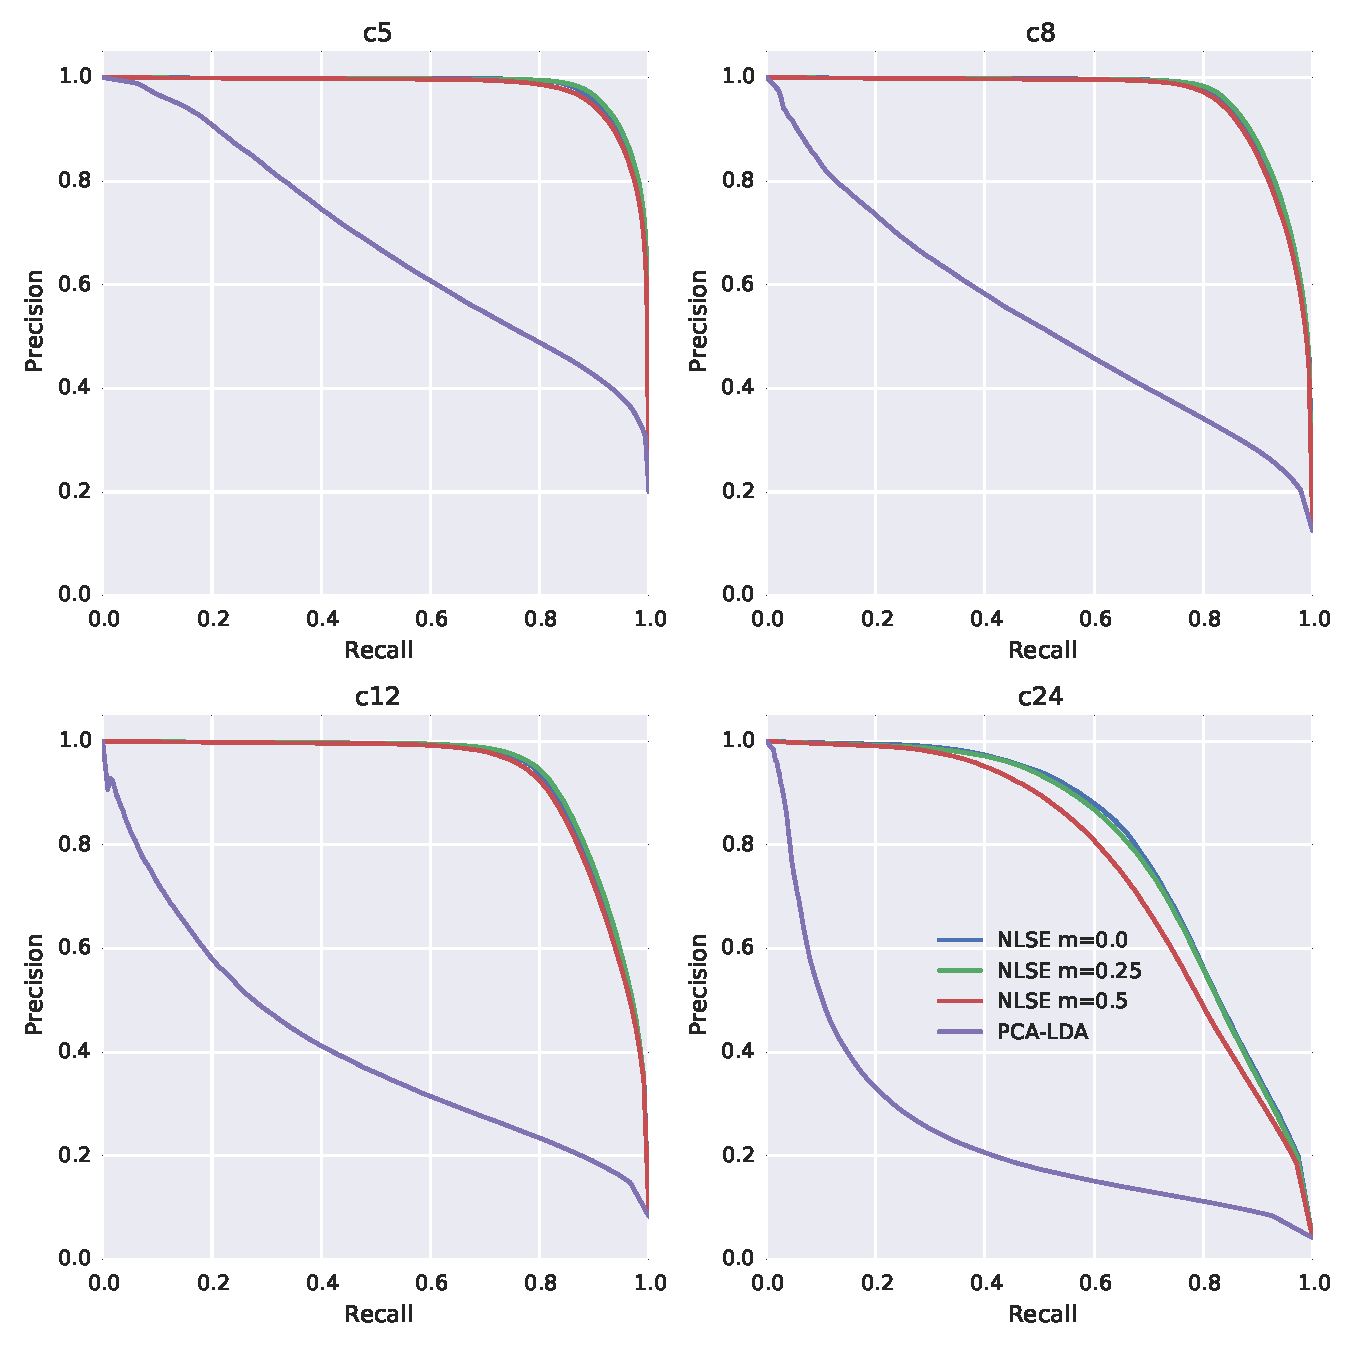
\includegraphics[width=\textwidth]{rp_curves.pdf}
\caption{Recall-Precision curves over the four instrument configurations.}
\label{fig:rp_curves}
\end{figure}

Given the classification accuracy and confusion matrices above, the performance gap between the NLSE and PCA-LDA models is unsurprising.
Still, it is interesting to consider what the shape of these recall-precision curves indicates.
The two characteristics to observe are the concavity of the contour and the ``knee'' at which it breaks downward.
In all instrument configurations, with the slight exception of ``c5'', the NLSE models and the PCA-LDA model exhibit opposite second-derivatives.
This behavior can be understood as the acceleration with which precision changes as a function of recall.
For the NLSEs, precision degrades slowly until reaching a crossover point, referred to here as the knee, where precision drops off rapidly.
The PCA-LDA model does the opposite, where precision drops quickly close to a query point, and slows as recall increases.
Therefore, as encouraged by the visualizations, the NLSEs contain better separated class clusters than the PCA-LDA embeddings.
Furthermore, the knee of a recall-precision curves belies an interesting region in the document space, indicating that the edge of a cluster has been reached.
This is a useful observation for determining early-stopping criteria in the display of ranked results, as well as identifying boundary regions in the embedding that may present interesting opportunities for sonic exploration.

Looking to differences between NLSEs, there are two variables to consider: instrument configuration and margin ratio.
For the first three instrument configurations, precision is roughly 100\% out past a recall of 0.6;
this can be understood as the top 60\% of results for a given query will correctly match that instrument.
In the final condition though, ``c24'', this break occurs just past a recall of 0.2, at which point other instrument samples would start to appear in the list of results.
This is still quite good from the perspective of precision at the top of the ranked list, but it illustrates the point at which the embedding space is beginning to get crowded.
A higher dimensional embedding might alleviate this at the expense of visualization, but would still be suitable for a retrieval system.
With respect to the margin ratio, the first three instrument conditions are again roughly equivalent, whereas ``c24'' begins to show more contrast between the embeddings.
In all conditions $\frac{m_s}{m_d} = 0.5$ yields the lowest performing NLSE, and is most pronounced in the final condition.
This is consistent with expectation, because the larger value of $m_s$ places de-emphasizes the tightness of instrument clusters, causing more overlap between the different classes.


\section{Conclusions}
\label{sec:conclusions}

In this chapter, an approach to building a computational model of timbre similarity was presented, which achieved three goals.
First, the system is able to automatically learn relevant signal level features, circumventing the challenge posed by the lack of a constructive definition of timbre.
Second, the resulting timbre space is semantically well-organized, as demonstrated by classification and ranked retrieval measures, and intuitive, based on a Euclidean notion of distance in a dimensionality that can be easily visualized.
Lastly, the space is quantitatively smooth, such that what confusions exist correspond to instrument families or other like sounds.
This was made possible by leveraging objective information about a collection of sound sources, eliminating the need for costly subjective ratings.
Together, this approach to learning a timbre space shows promise for visualization and user-facing applications, such as the search and navigation of large sound libraries.

That said, there is considerable future work to be considered.
All evaluation performed here is quantitative, and arguably disconnected from all subjective experience.
User studies would serve to further investigate the ideas of perceptual smoothness and if or how is obtained by the learned space.
Efforts to analyze the learned features may further help elucidate the latent factors that contribute to the percept of timbre.
Additionally, though this approach is able to make use of objective instrument taxonomies, any similarity space obtained through pairwise comparisons is always limited by the range of inputs considered.
Therefore, in order to obtain a more general timbre space, a much wider set of sound sources would need to be considered.
Conversely, the intended use case of such a system may provide a constrained palette with which to operate, e.g. instrument sounds for recording engineers and environmental sounds for acoustic ecologists.
Finally, there are at least two other ways the sound source information could be used to train a system in a supervised manner.
One, it may be advantageous to obtain subjective pairwise ratings not between all possible sounds, but rather groups or classes of sounds.
These pairwise ratings could be used to train a system with soft, continuous-valued similarity ratings, rather than the binary comparison scores used here.
Two, rather than defining an entire class to be similar, a hybrid approach to similiarity based on distance-based neighborhoods in the input space constrained to a single class may also lead to interesting embeddings.
It is unlikely such an embedding would exhibit spherical clusters as was produced here, but points are likely to be more uniformly distributed, or diffuse, in space.
